\documentclass{beamer}

\usepackage[utf8]{inputenc}
\usecolortheme{beaver}
\usepackage{caption}
\usepackage{subcaption}
\usepackage{mathtools}
\usepackage{todonotes}
\usepackage{amsmath}
\usepackage{bm}
\usepackage{listings}
\usepackage{ragged2e}
\usepackage{fancyvrb}
\usepackage{titlecaps}
\usepackage{hyperref}

\Addlcwords{for a is but and with of in as the etc on to if}

\def\ci{\perp\!\!\!\!\!\perp}

\tikzstyle{latent} = [ draw, circle, inner sep = 2pt, minimum size = 0.65cm ]
\tikzstyle{observed} = [ draw, rectangle, inner sep = 2pt, minimum size = 0.65cm ]

\newtheorem{proposition}{Proposition}

\setbeamertemplate{section in toc}{\inserttocsectionnumber.~\inserttocsection}
\usetheme{Boadilla}
\makeatletter
\setbeamertemplate{footline}{%
    \leavevmode%
    \hbox{%
        \begin{beamercolorbox}[wd=.3\paperwidth,ht=2.25ex,dp=1ex,center]{author in head/foot}%
            \usebeamerfont{author in head/foot}\insertshortauthor\expandafter\beamer@ifempty\expandafter{\beamer@shortinstitute}{}{~~(\insertshortinstitute)}
        \end{beamercolorbox}%
        \begin{beamercolorbox}[wd=.55\paperwidth,ht=2.25ex,dp=1ex,center]{title in head/foot}%
            \usebeamerfont{title in head/foot}\insertshorttitle
        \end{beamercolorbox}%
        \begin{beamercolorbox}[wd=.15\paperwidth,ht=2.25ex,dp=1ex,right]{date in head/foot}%
            \usebeamerfont{date in head/foot}\insertshortdate{}\hspace*{2em}
            \insertframenumber{} / \inserttotalframenumber\hspace*{2ex} 
        \end{beamercolorbox}}%
        \vskip0pt%
    }
\makeatother

\begin{document}

\title[]{Papers}
\author [] {Ankur Ankan}
\date{}
\maketitle

\begin{frame}
	\frametitle{\titlecap{Conditional Independence (CI) Test for combination of discrete, ordinal, and continuous variables}}
	\begin{figure}
		\centering
		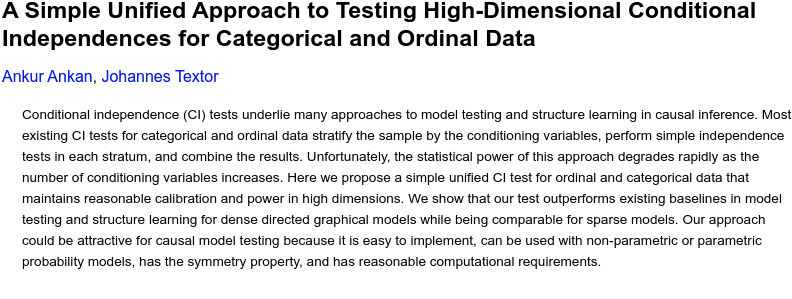
\includegraphics[scale=0.4]{imgs/ankan_textor}
		\caption*{}
	\end{figure}
	\vspace{-2em}
	\begin{itemize}
		\item Paper describes only combination of ordinal and categorical variables.	
	\end{itemize}
\end{frame}

\begin{frame}
	\frametitle{\titlecap{CI Test: Possible Applications}}
	\begin{itemize}
		\item \textbf{Constraint-Based Structure Learning:} Systematically searches for CI in data to construct structure. E.g., PC, FCI.
			$$ \textit{ If } X \ci Y \mid \bm{Z} \subseteq \textit{neig}(X, Y)  \implies \textit{No edge between X and Y} $$
		\item \textbf{Model Testing:} If the model structure implies $ X \ci Y \mid Z $, then that should hold true in the data.
		\item \textbf{Effect Size:} Can be used to show the edge weight between variables.
	\end{itemize}
\end{frame}

\begin{frame}
	\frametitle{\titlecap{CI Test: Main Idea}}
	\begin{enumerate}
		\item Residualizaton approach.
		\item Similar to partial correlation for continuous variables.
		\item For testing whether $ X \ci Y \mid Z $ using partial correlation:
			\begin{enumerate}
				\item Train two estimators: $ E_X = X \sim Z $ and $ E_Y = Y \sim Z $.
				\item Make predictions using these estimators: $ \hat{X} = E_X(Z) $ and $ \hat{Y} = E_Y(Z) $.
				\item Compute residuals: $ R_X = X - \hat{X} $ and $ R_Y = Y - \hat{Y} $.
				\item Do a correlation test between $ R_X $ and $ R_Y $.
			\end{enumerate}
		\item Proposed test:
			\begin{itemize}
				\item No simple residual definition for ordinal and categorical variables. We use LS-Residuals \footnote{Li, Chun, and Bryan E. Shepherd. "A new residual for ordinal outcomes." Biometrika 99.2 (2012): 473-480.}
				\item The correlation test can give incorrect results \footnote{Shah, Rajen D., and Jonas Peters. "The hardness of conditional independence testing and the generalised covariance measure." (2020): 1514-1538.}. We give new test statistics.
			\end{itemize}
	\end{enumerate}
\end{frame}

\begin{frame}
	\frametitle{\titlecap{CI Test: Proposed Algorithm}}
	\begin{enumerate}
		\item If either $ X $ or $ Y $ are non-binary categorical, dummy encode them.
		\item Train two probability estimators $ p_x = \bm{x} \sim \bm{z} $ and
			$ p_y = \bm{y} \sim \bm{z} $.
			\begin{itemize}
				\item Any estimator that gives valid residuals can be used.
			\end{itemize}
		\item Make probability predictions:
			$ \hat{p}(\bm{x}) = p_x(\bm{z}) $ and $ \hat{p}(\bm{y}) = p_y(\bm{\bm{z}}) $.
		\item Compute LS-Residuals:
			$$ R_{y_i | z_i} = \hat{p}(Y < y_i | Z=z_i) - \hat{p}(Y>y_i|Z=z_i) $$
		\item Use residuals to compute test statistics.
			$$ Q = \frac{1}{n} (d \times \hat{\Sigma}_d^{-1} \times d^T) $$
			$$ d = R_{x|z} R_{y|z} $$
		\item Under null, $ Q $ is $ \chi^2 $ distributed.
		\item Canonical correlation between residuals gives us the Cramer's V.
	\end{enumerate}
\end{frame}

\begin{frame}
	\frametitle{\titlecap{CI Test: Emprical Result}}
		\begin{figure}
		\begin{subfigure}{.33\textwidth}
			\centering
			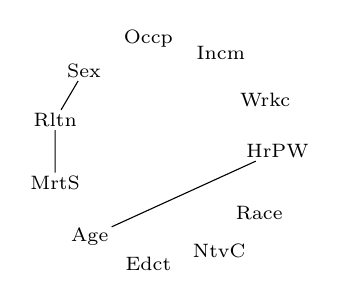
\begin{tikzpicture}[scale=1.2]
				\tikzstyle{every node}=[align=center, inner sep=1pt]
				\scriptsize
				\node (hrpw) at (0:1.2cm) {HrPW};
				\node (race) at (-33:1.2cm) {Race};
				\node (ntvc) at (-61:1.2cm) {NtvC};
				\node (edct) at (-98:1.2cm) {Edct};
				\node (age) at (-131:1.2cm) {Age};
				\node (mrts) at (-164:1.2cm) {MrtS};
				\node (rltn) at (-196:1.2cm) {Rltn};
				\node (sex) at (-225:1.2cm) {Sex};
				\node (occp) at (-262:1.2cm) {Occp};
				\node (incm) at (-300:1.2cm) {Incm};
				\node (wrkc) at (-333:1.2cm) {Wrkc};
				\draw [] (sex) -- (rltn);
				\draw [] (mrts) -- (rltn);
				\draw [] (hrpw) -- (age);
			\end{tikzpicture}
			\caption{}
		\end{subfigure}%
		\begin{subfigure}{.33 \textwidth}
			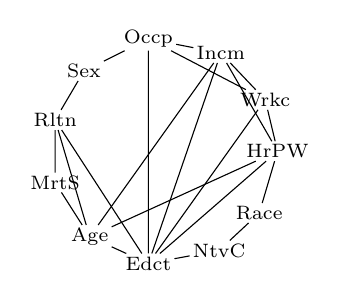
\begin{tikzpicture}[scale=1.2]
				\tikzstyle{every node}=[inner sep=1pt, align=center]
				\scriptsize
				\node (hrpw) at (0:1.2cm) {HrPW};
				\node (race) at (-33:1.2cm) {Race};
				\node (ntvc) at (-61:1.2cm) {NtvC};
				\node (edct) at (-98:1.2cm) {Edct};
				\node (age) at (-131:1.2cm) {Age};
				\node (mrts) at (-164:1.2cm) {MrtS};
				\node (rltn) at (-196:1.2cm) {Rltn};
				\node (sex) at (-225:1.2cm) {Sex};
				\node (occp) at (-262:1.2cm) {Occp};
				\node (incm) at (-300:1.2cm) {Incm};
				\node (wrkc) at (-333:1.2cm) {Wrkc};

				\draw [] (hrpw) -- (race) -- (ntvc) -- (edct) -- (age) -- 
					(mrts) -- (rltn) -- (sex) -- (occp) -- (incm) -- (wrkc) -- (hrpw);

				\draw [] (hrpw) -- (incm) -- (age) -- (hrpw);

				\draw [] (wrkc) -- (edct) -- (occp) -- (wrkc);

				\draw [] (edct) -- (rltn) -- (age);

				\draw [] (hrpw) -- (edct) -- (incm);
			\end{tikzpicture}
			\caption{}
		\end{subfigure}%
		\begin{subfigure}{0.33\textwidth}
			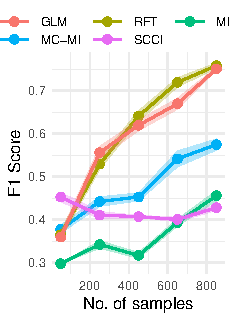
\includegraphics[scale=0.7]{imgs/adult_F1.pdf}
			\caption{}
		\end{subfigure}
			\caption{Structure learning on Adult Income dataset:
			(a) Using chi-squared test (b) Using our test with
			Random Forest estimator (c) F1 Score of whether
			correlation variables in the data are d-connected in
			the learned structure.}
		\end{figure}
\end{frame}

\begin{frame}
	\frametitle{\titlecap{Probabilistic Programming Framework for exact inference}}
	\begin{figure}
		\begin{subfigure}{\textwidth}
			\centering
			
\includegraphics[scale=0.4]{imgs/pan_shaikhha.png}
		\end{subfigure}
		\begin{subfigure}{\textwidth}
			\centering
			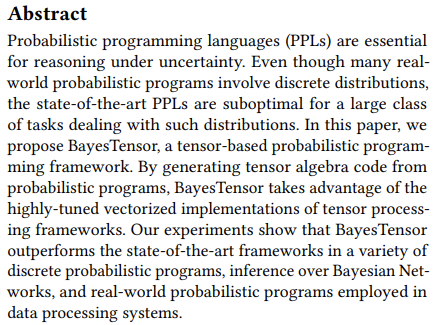
\includegraphics[scale=0.4]{imgs/pan_shaikhha_abstract.png}
		\end{subfigure}
	\end{figure}
\end{frame}

\begin{frame}
	\frametitle{\titlecap{Variable Elimination for discrete BNs}}
	\begin{columns}
		\begin{column}{0.3 \textwidth}
			\begin{figure}
				\centering
				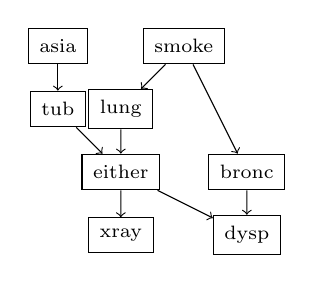
\begin{tikzpicture}[scale=0.8]
					\tikzstyle{every node}=[inner sep=1pt, align=center]
						\scriptsize
						\tikzstyle{every node}=[draw, rectangle, inner sep=4pt, align=center]
						\node (asia) at (0, 0) {asia};
						\node (tub) at (0, -1) {tub};
						\node (smoke) at (2, 0) {smoke};
						\node (lung) at (1, -1) {lung};
						\node (either) at (1, -2) {either};
						\node (xray) at (1, -3) {xray};
						\node (bronc) at (3, -2) {bronc};
						\node (dysp) at (3, -3) {dysp};

						\draw [->] (asia) -- (tub);
						\draw [->] (tub) -- (either);
						\draw [->] (either) -- (xray);
						\draw [->] (either) -- (dysp);
						\draw [->] (smoke) -- (lung);
						\draw [->] (lung) -- (either);
						\draw [->] (smoke) -- (bronc);
						\draw [->] (bronc) -- (dysp);
				\end{tikzpicture}
			\end{figure}
		\end{column}
		\begin{column}{0.7 \textwidth}
			\center \textbf{Inference:} $ P(either) = \sum_{\bm{X} - \{either\}} P(\bm{X}) $
			\center \textcolor{red}{Computationally intractable!}
		\end{column}
	\end{columns}
	\vspace{0.5em}
	\begin{enumerate}
		\item \textbf{Network Pruning}:
			\begin{equation*}
				\begin{split}
					P(lung) & \implies \textit{Remove tub and asia as d-separated.} \\
					P(lung \mid either, bronc) & \implies \textit{Remove xray and dysp as cond. d-sep.}
				\end{split}
			\end{equation*}
		\item \textbf{Elimination order}: Push the summation inside. The order of summation decides computational cost.
			``opt\_einsum'' provides some efficient algorithms.
			$$ P(either, bronc) = \sum \cdots \sum_{xray} P(xray \mid either) \sum_{dysp} P(dysp \mid either, bro.) $$
	\end{enumerate}

\end{frame}
\begin{frame}
	\frametitle{\titlecap{Main Idea}}
	\begin{enumerate}
		\item Proposes a better way to do network pruning.
		\item Takes in the network and gives out an einsum expression.
	\end{enumerate}
\end{frame}

\begin{frame}
	\frametitle{\titlecap{MAG and PAG}}
\end{frame}

\begin{frame}
	\frametitle{\titlecap{Learning from combination of interventional and observational datasets}}
\end{frame}

\begin{frame}
	\frametitle{\titlecap{Transportability}}
	\url{https://www.annualreviews.org/doi/pdf/10.1146/annurev-statistics-042522-103837}
\end{frame}
\end{document}
